\section{Auswertung}
\label{sec:Auswertung}

\subsection{Kontrast}
Zunächst wird der Kontrast berechnet.
Die entsprechenden Messwerte finden sich in \autoref{tab:kontrast}.
Nun lässt sich mit \autoref{eq:kontrast} der Kontrast berechnen. Dabei wird die Intensität gleichgesetzt mit der Spannung.
Die Ergebnisse finden sich in der rechten Spalte von \autoref{tab:kontrast}.
\input{build/kontrast.txt}
Als Fit wurde die Funktion 
\begin{equation*}
    f(x) = A \cdot \sin(2 x - \delta)
\end{equation*}
angenommen. Dies ist wegen der Proportionalität aus \autoref{eq:kontrast2} gerechtfertigt.
\begin{figure}
    \centering
    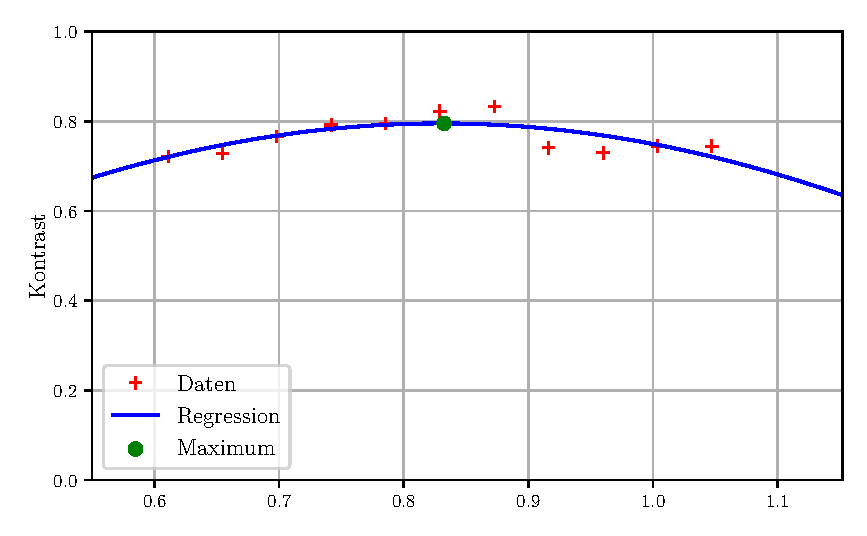
\includegraphics[width = 0.7 \linewidth]{build/Kontrast.pdf}
    \caption{Fit der Theoriekurve an die Messdaten.}
    \label{fig:plot1}
\end{figure}
Der Fit ist in \autoref{fig:plot1} zu sehen.
Für die Variablen ergibt sich $\delta = 0.0877 \pm 0.038$ und $A = 0.8 \pm 0.0085$.
Hieraus ergibt sich das theoretische Maximum von $K = 0.8$ bei einem Winkel von $47.69°$.

\subsection{Brechungsindex Glas}
Nun wird der Brechungsindex von Glas bei einer Rotation von $11°$ und einer Dicke von $T = 1 \unit{\milli\meter}$ berechnet.
Die Messdaten sind in \autoref{tab:glas} zu finden.
Mithilfe von Formel \autoref{eq:nluft} lässt sich nun der Brechungsindex bestimmen.
Auch diese Ergebnisse sind in \autoref{tab:glas} zu finden.
\input{build/n_glas.txt}

\subsection{Brechungsindex Luft}
Die Messdaten der drei Messreihen sind in \autoref{tab:luft} zu finden.
\input{build/n_luft.txt}
Hier sind auch die berechneten Brechungsindizes zu finden.
Diese wurden nach \autoref{eq:n_Glas} berechnet.